\chapter{Interferences between coherent sources}
\label{ch:Investigation of a coherent source}



%Let's consider 2 


A Gaussian beam is fully characterized by its waist and phase (radius of curvature $R$ in Gaussian beam theory) in a given plane. When varying $R$ in the plane $z=0$, where the waist is $w$, the "focus" is no longer located at $z=0$, but at position $z_0$, with a corresponding waist $w_0$. The question we ask is: is it possible to reach arbitrary values of $z_0$ when changing $R$?

\begin{figure}[H]
\centering
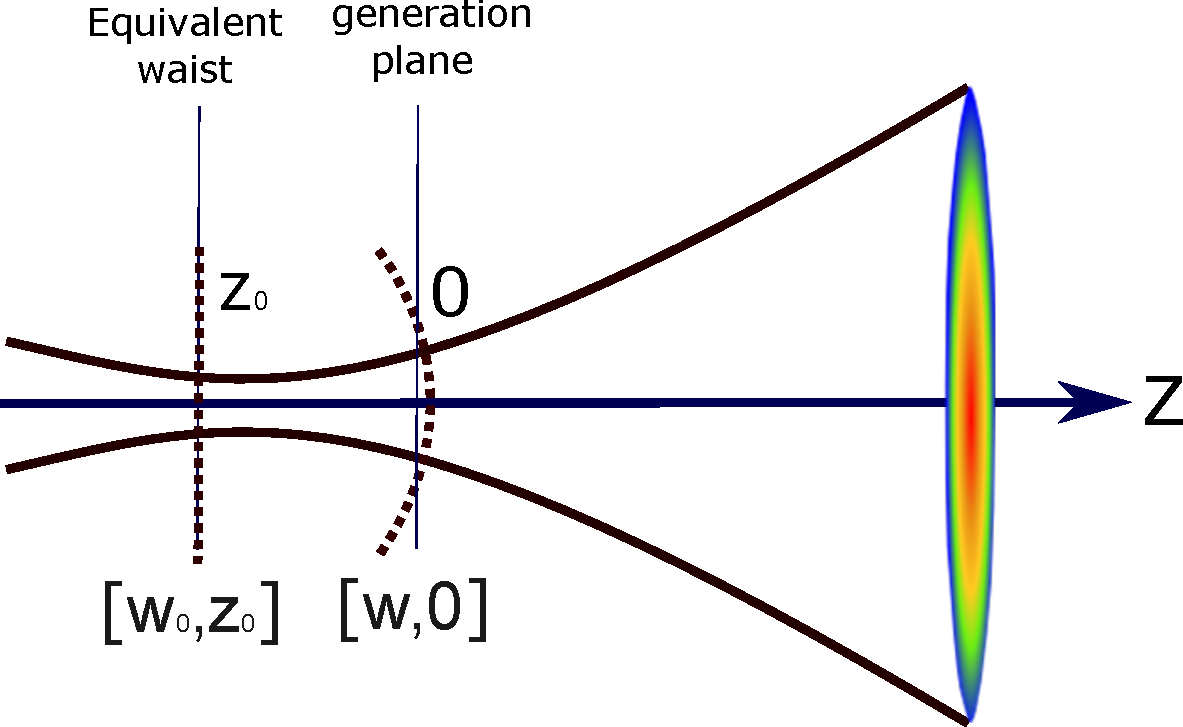
\includegraphics[width =0.5\textwidth]{../annexe/images/GaussianBeamDef.pdf}\\
\caption{\label{fig:GaussianBeamDef} Representation of a Gaussian pulse}
\end{figure}

\noindent In Gaussian beam theory, the phase radius of curvature is defined by:
$$
R = -z_0 - \frac{Z_r^2}{z_0}
$$

\noindent Where $Z_R = \frac{\pi w_0^2}{\lambda}$ is the Rayleigh length.\\

\noindent That first relation does not provide enough information because two different values of $z_1$ (one very small, one very big) can lead to the same $R$. In other words, this $z_0\rightarrow R$ relation does not constitute a bijection of $\mathbb{R}^*$ in $\mathbb{R}$. We use another relation on the waists:

\begin{equation}
\label{eq:relationWaist}
w =w_0\sqrt{1+\frac{z_0^2}{Z_R^2}}
\end{equation}


\noindent Replacing $Z_R$ by its definition in~\ref{eq:relationWaist}, we derive the following equation:

\begin{equation}
(w_{0}^2)^2 - w^2(w_{0}^2) + z_{0}^2\frac{\lambda^2}{\pi^2} =0
\end{equation}

\noindent The discriminant $\Delta$ of that equation should be positive in order to find a solution for $w_0$, which ever value we impose on $w_0$. Moreover, the minimum waist is always at the position of flat phase such that we will always keep the smallest (positive) solution of that equation. A solution for $(w_0^2)$ exists if, and only if:

\begin{equation}
\Delta = w^4 - 4z_{0}^2\frac{\lambda^2}{\pi^2} \ge 0
\end{equation}

\noindent that is to say 
$$
|z_{0}| \le \frac{w^2\pi}{2\lambda}
$$

\noindent This means that which ever the phase we associate with a source of given waist $w$ and wavelength $\lambda$, the equivalent waist (within the theory of Gaussian beams) is always be in an interval $[- \frac{w^2\pi}{2\lambda}, \ \ \frac{w^2\pi}{2\lambda}]$. This means a harmonic source can not be equivalent to a Gaussian beam arbitrarily far from the focus position where the interaction takes place. Indeed, $R$ can be extremely large if $z << Z_R$ or $z >>Z_r$, and will be smaller for intermediate values. Therefore, another approach is to say: if $R$ would be arbitrarily large, the beam could be considered very far from the position of its waist. Therefore, it would be almost collimated. But a collimated beam with a very small waist should diverge extremely quickly, which is in contradiction with the collimation. Necessarily, if $R$ is large this means the waist is located within the Rayleigh length.

\subsubsection{3 sources in vertical plane:}

In \textit{Matlab}, we use the analytical expression of a Gaussian beam\cite{CoursForget} and explore the interference pattern resulting from 3 sources positioned vertically along the $r$ axis as represented in Fig~\ref{fig:3sources}.
Each Gaussian beam indexed by $i$ is defined by the variables $[w_{0i},z_i]$ where $w_{0i}$ is the waist at focus, and $z_i$ the position of the focus.

\begin{figure}[H]
\centering
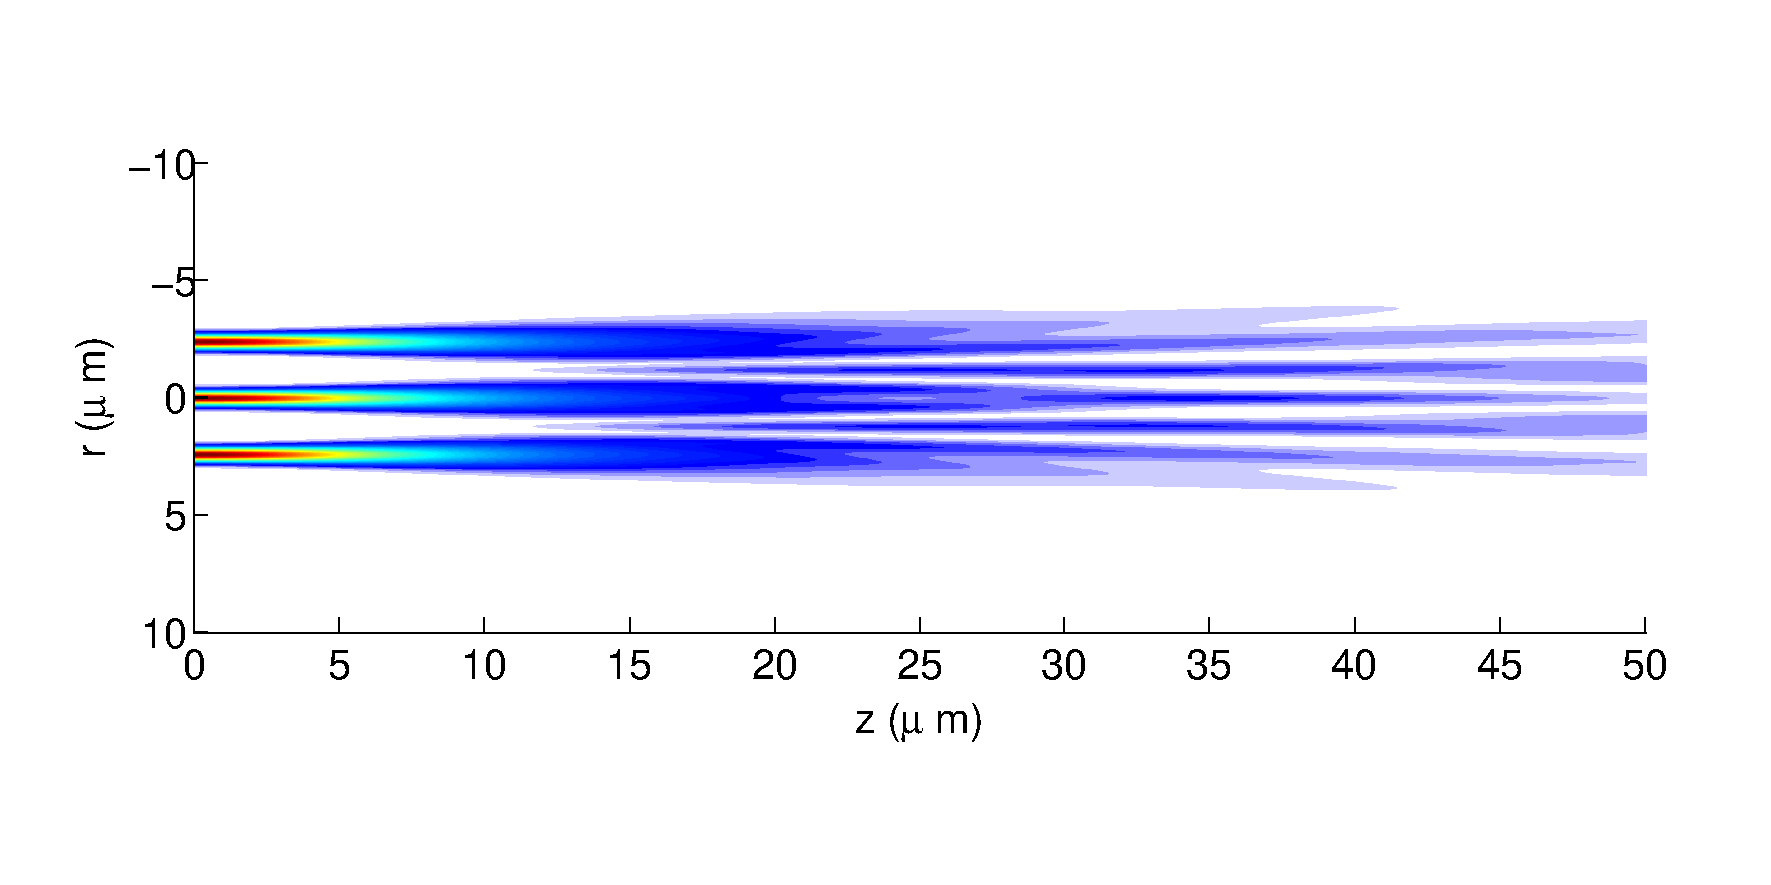
\includegraphics[width =\textwidth]{../annexe/images/3sources.pdf}\\
\caption{\label{fig:3sources} Representation in the plane $(r,z)$ where $z$ indicates the direction of the resulting intensity where $w_{0i} = 400\,\mathrm{nm}$,$z_{0i} =0$, $r_{01} = -r_{03} = 2.4\,\mathrm{\mu m}$, $r_{02}=0$ and $\lambda = 80\,\mathrm{nm}$}
\end{figure}

\noindent In this configuration where $r_{01} = -r_{03}$, the $n^{th}$ diffracted interfringe is given by :

\begin{equation}
\label{eq:interfrange vertical sources}
\Theta_n = n\frac{\lambda}{|r_{01}|}
\end{equation}

%Thefore, to resolve interferences ($\delta \theta > 1 \mathrm{mRad}$ typically on our detector) we need 

\noindent Using the analytical formulas at position $z>> Z_R$, we can extract an interference pattern as the result of this 3 source configuration and the angular interfringe does correspond to that given by Eq~\ref{eq:interfrange vertical sources}. The simplest way to retrieve the distance between the sources $r_1$ is to Fourier transform the result. The main non-zero angular frequency will therefore correspond to:
\begin{equation}
f_{\theta} = \frac{r_{01}}{\lambda}
\end{equation}

\noindent It is therefore convenient to replace $f_{\theta}$ by $f_{\theta}\lambda$ after computing the Fourier signal to have the maximum at exactly $r_{01}$. In Fig~\ref{fig:3sourcesGaussianSimus}, we look at the influence of the intensity interference pattern on the Fourier transform when changing one parameter in this 3-source configuration. Here the beams $i = 1$ and $i=3$ are taken symmetric.
The dimensions are given  in $\lambda_0$ unit, where $\lambda_0 = 800\,\mathrm{nm}$ while each Gaussian beam is defined for the $10^{th}$ harmonic ($\lambda = 80\,\mathrm{nm}$)

\begin{figure}[H]
\centering
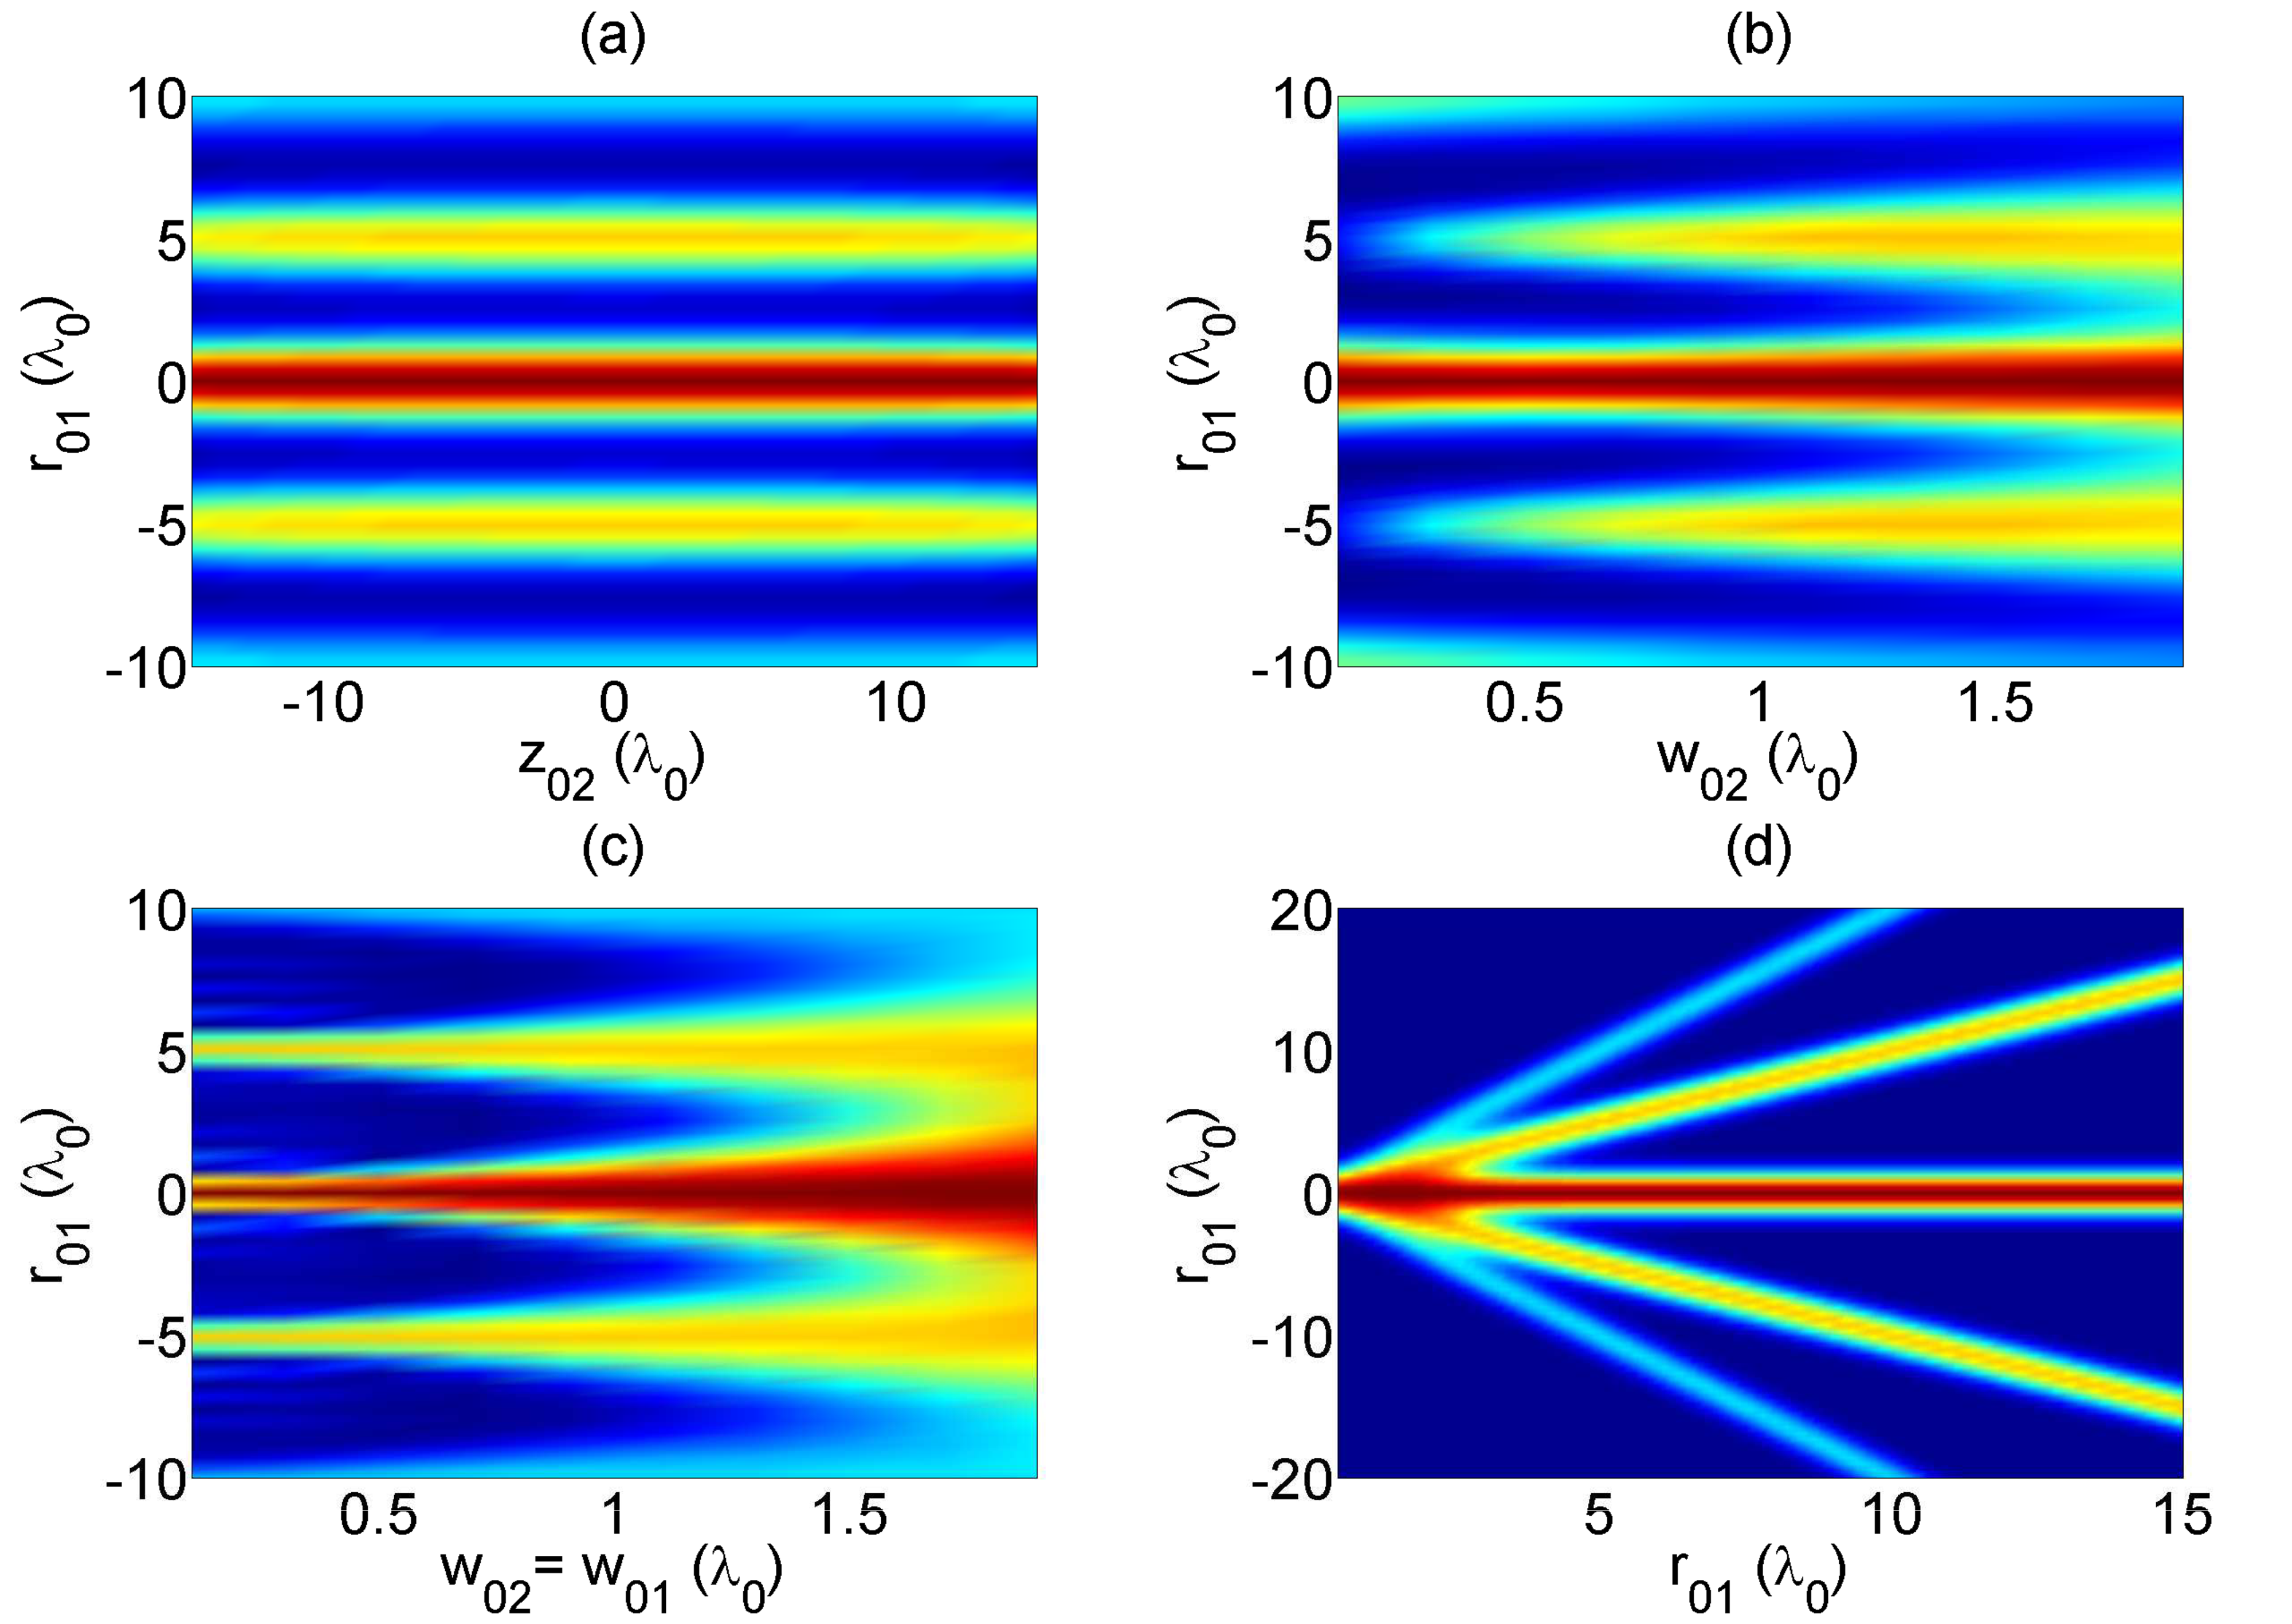
\includegraphics[width =15cm]{../annexe/images/3sourcesGaussianSimus.pdf}\\
\caption{\label{fig:3sourcesGaussianSimus} Fourier transform of intensity interference pattern for harmonic H10 ($\lambda = 80\,\mathrm{nm}$). Initial conditions are $z_{0i} = 0$, $w_{0i}=\lambda_0$ and $r_{01} = 5\lambda_0$. We then vary one parameter: (a) influence of central source defocus (b) influence of central source waist (c) influence of global waist variation (d) influence of satellite sources distance $r_{01}$ }
\end{figure}

%\subsubsection{2 sources aligned on $z$ axis:}
%
%\noindent 2 sources aligned on the $z$ axis will generate a ring pattern in the far field with an interfrange that will depend on the parameter $n$. The interferences are constructive when $n$ is interger and detructive when $n$ is an integer and a half. 
%
%\begin{equation}
%\Theta_n = \sqrt{2(1-\frac{n\lambda}{(z_2 - z_1)})}
%\end{equation}
%
%\noindent This simple expression actually leads to conter intuitive results. Indeed, for $a\sim 0.5\lambda$, destructibe interferences will appear near $\theta = 0$. We verify this by propagating 2 Gaussian beam and find the window in wich this "rings" would be observerble is extremely narrow. 
%
%\begin{figure}[H]
%\centering
%\fbox{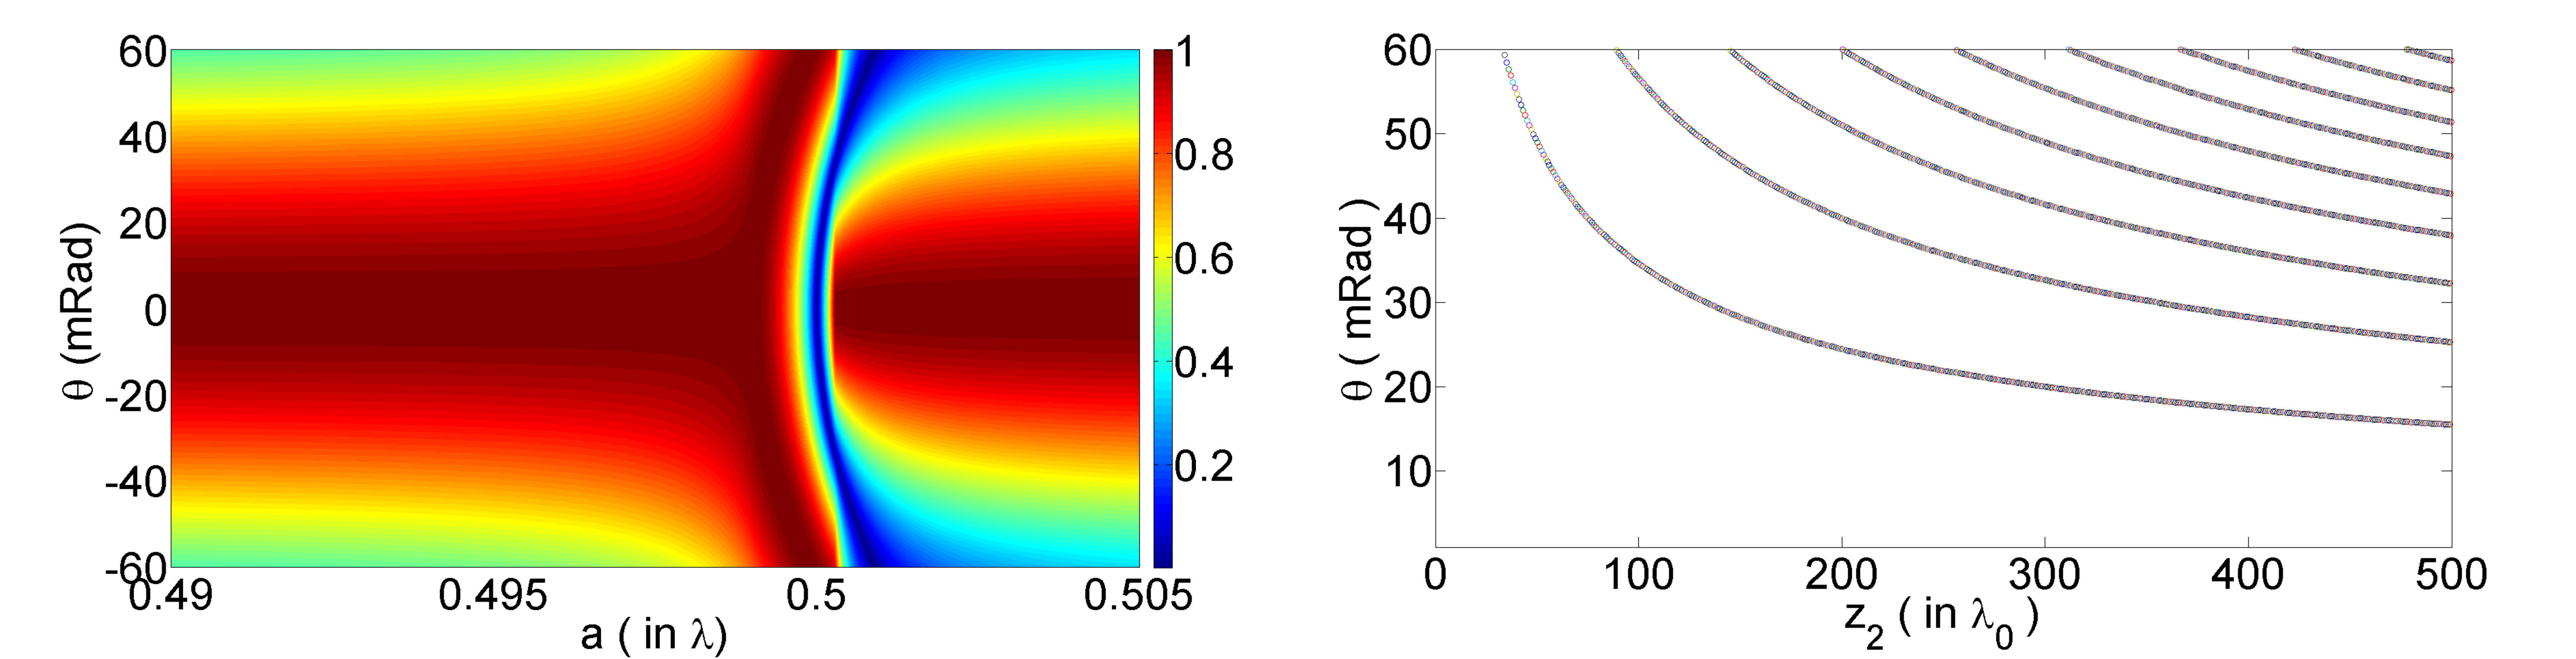
\includegraphics[width =15cm]{../chapitre6/images/2sourcesGaussianFormulaPlots.pdf}}\\
%\caption{\label{fig:2sourcesGaussianFormulaPlots} Conditions de simulation for H10: (a) $w_1 = w_2 = 0.5\lambda_0$ . Here $\lambda_0 = 800\mathrm{nm}$. $z_1 = 0$. (a) zoom on singularity near $a = 0.5 \lambda$, (b) evolution of destructive interfrences ($n$ is taken between $1$ and $1000$ $+1/2$) using formula}
%\end{figure}
%
%
%
%\begin{figure}[H]
%\centering
%\fbox{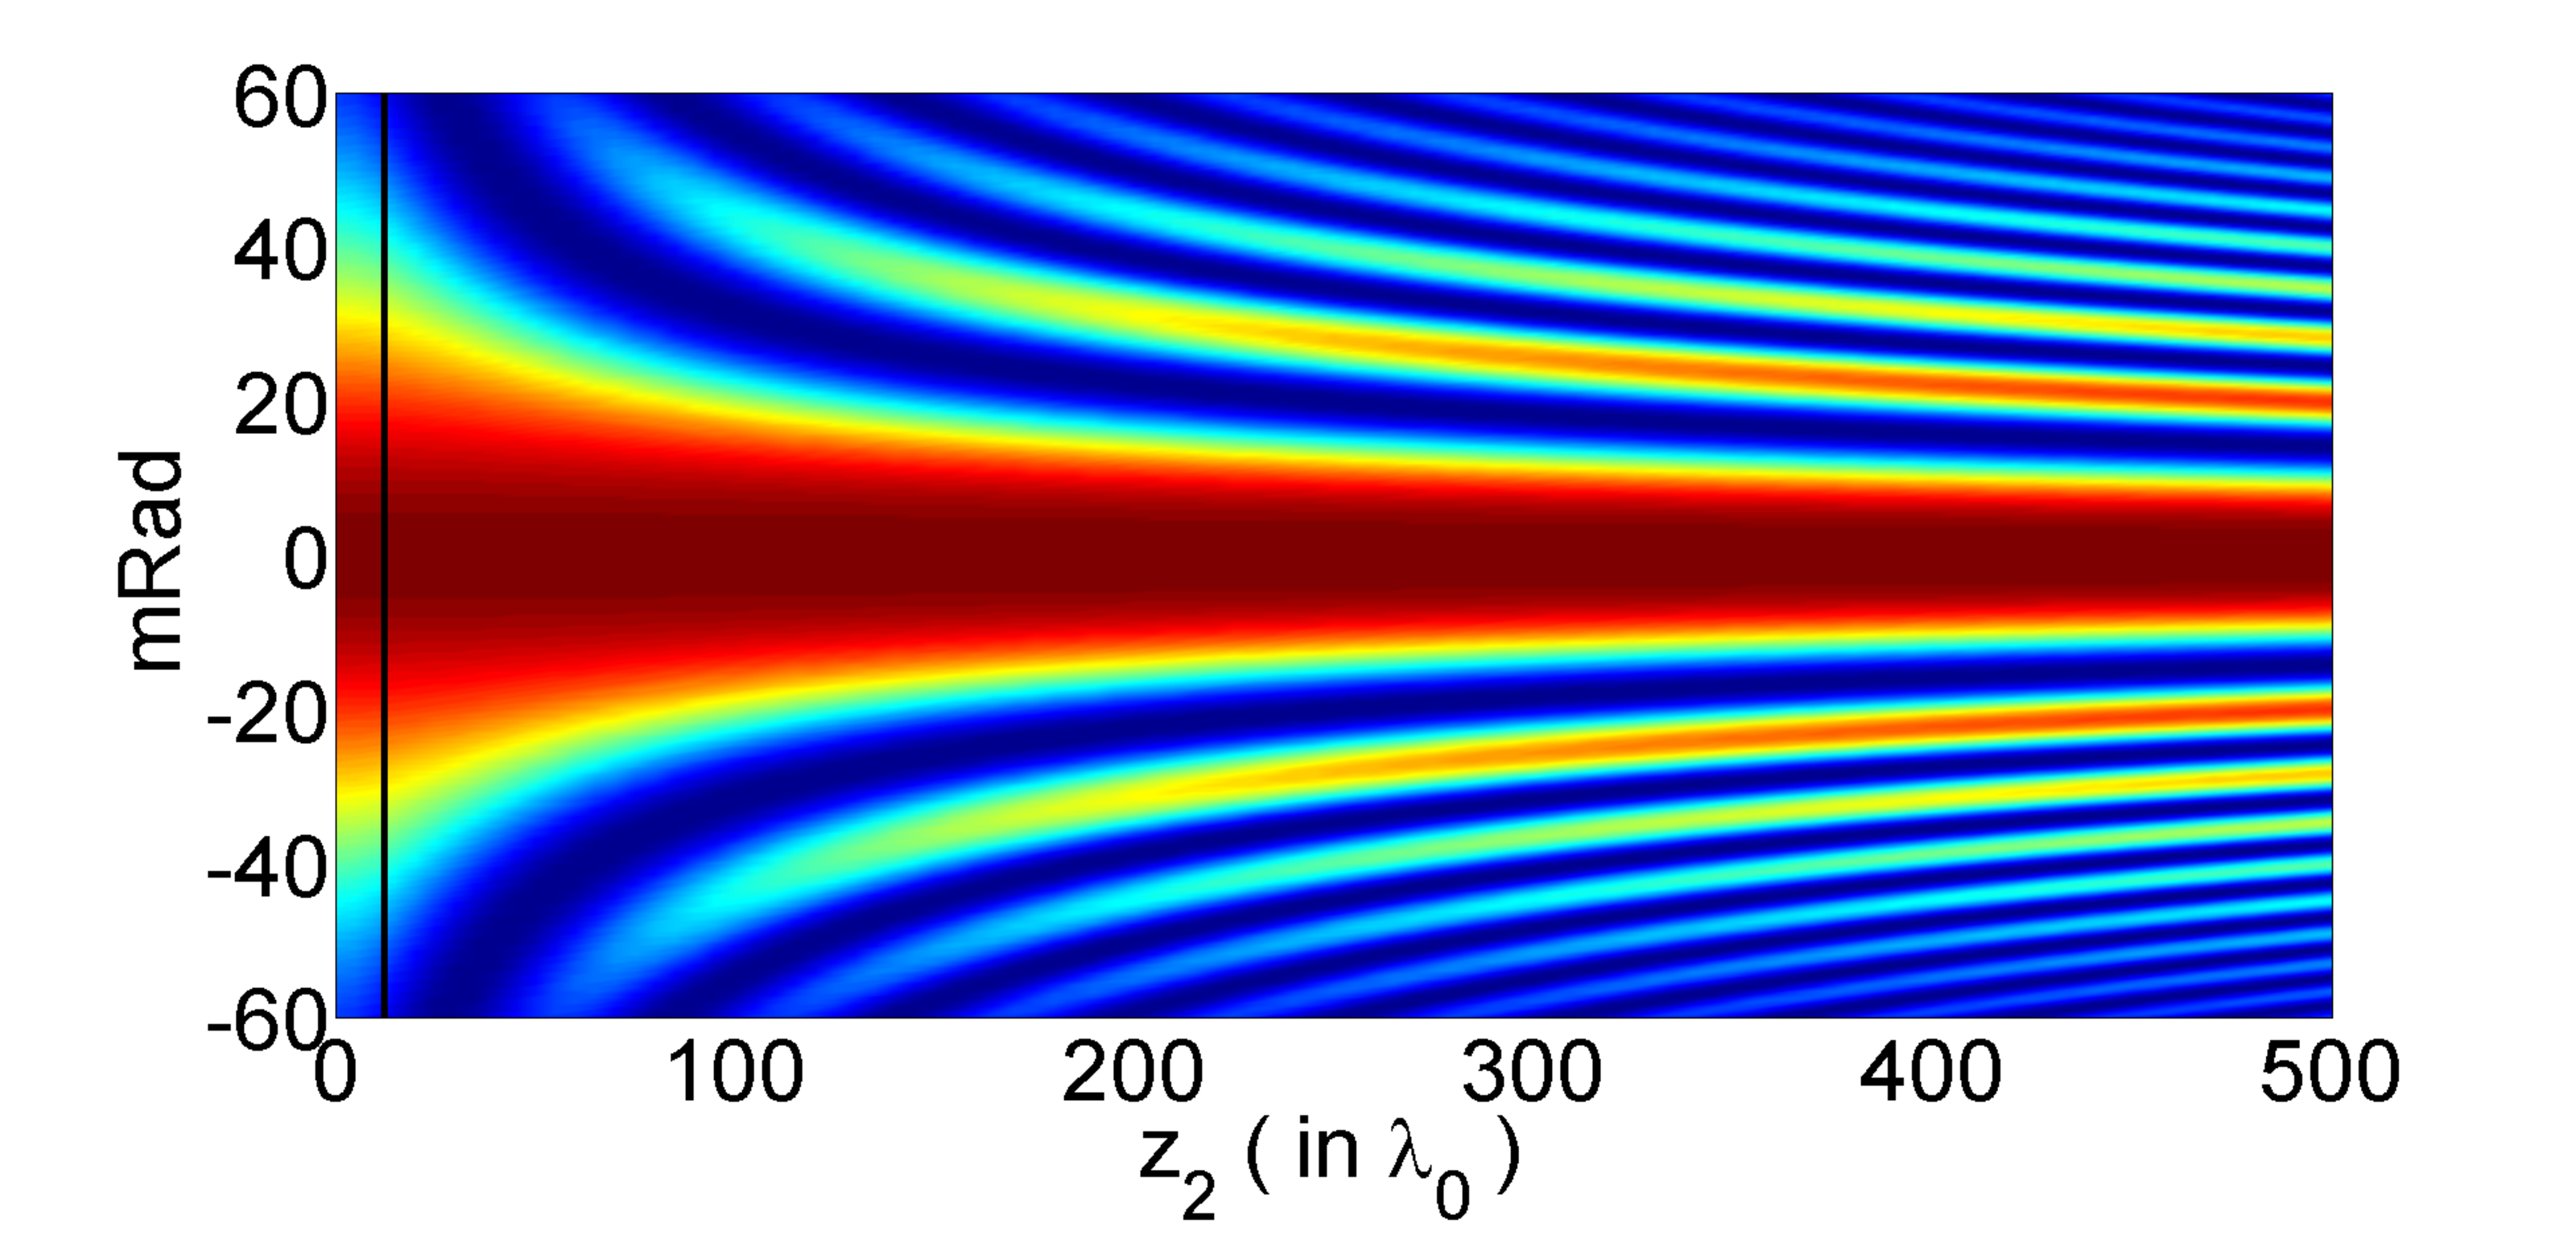
\includegraphics[width =15cm]{../chapitre6/images/2sourcesGaussianSimus.pdf}}\\
%\caption{\label{fig:2sourcesGaussianSimus} Conditions de simulation for H10: (a) $w_1 = w_2 = 0.5\lambda_0$ The relative position $z_2$ is increased linearly from $0$ to $500\lambda_0$. Here $\lambda_0 = 800\mathrm{nm}$. The black line represents the limite in $z$ offset induced by a possible phase modulation of the beam.}
%\end{figure}
%
%As a conclusion, interferences between 2 sources such as ROM and CWE are posssible only if the sources are very distant wich is not the case. 







